\documentclass[14pt]{extarticle}
\usepackage[
left=25mm,
top=20mm,
right=15mm,
bottom=20mm,
]{geometry}

%\usepackage{graphicx}
\usepackage[pdftex]{graphicx}
\usepackage[utf8x]{inputenc}
\usepackage[russian]{babel}
\usepackage[T1]{fontenc}
\usepackage{float}
\usepackage{listings}
\usepackage{cite}
\usepackage{hyperref}
\usepackage{etoolbox}
\usepackage{indentfirst}
\usepackage[linesnumbered,boxed]{algorithm2e}
\sloppy

\lstdefinelanguage{llang}{
keywords={skip, do, while, read, write, if, then, else},
sensitive=true,
basicstyle=\small,
commentstyle=\scriptsize\rmfamily,
keywordstyle=\ttfamily\underbar,
identifierstyle=\ttfamily,
basewidth={0.5em,0.5em},
columns=fixed,
fontadjust=true,
literate={->}{{$\to$}}1
}

\lstset{
language=llang
}
\makeatletter
%\renewcommand{\@biblabel}[1]{#1.} % Заменяем библиографию с квадратных скобок на точку:
\makeatother
\gappto\captionsrussian{\renewcommand{\contentsname}{Оглавление}}
\renewcommand\baselinestretch{1.5}
\renewcommand{\lstlistingname}{Листинг}

\begin{document}

\begin{titlepage}
\thispagestyle{empty}
\def\baselinestretch{1.0}
\begin{center}
	{САНКТ-ПЕТЕРБУРГСКИЙ ГОСУДАРСТВЕННЫЙ УНИВЕРСИТЕТ \\ \vskip 0.3em {\large Математико-механический факультет \\ \vskip 0.7em{\large Кафедра системного программирования \\}}}
    \vspace*{0.15\textheight}
    {\large Поздин Дмитрий Евгеньевич}
    
    \vskip 2em
    {\huge Декомпиляция выражений по байт-коду JVM}
    
    \vskip 1em
    {\large Курсовая работа} \\
    \vskip 2em
    {\normalsize \raggedleft 
    Допущена к защите.\\
    Зав. кафедрой:\\
    д.ф.-м.н., проф. А.Н. Терехов
    \\[3em]
    Научный руководитель:\\
    к.ф.-м.н. Д.Ю. Булычев
    \\[3em]
    %Рецензент:\\
    %Неизвестно \\
    \vspace*{0.08\textheight}
    {\centering Санкт-Петербург \\ 2013}
    }
\end{center}
\end{titlepage}

\tableofcontents
\thispagestyle{empty} 
\pagebreak

\iffalse
\documentclass[a4paper, 12pt]{article}
\usepackage[
left=25mm,
top=20mm,
right=25mm,
bottom=20mm,
]{geometry}
\usepackage{mathtext}
\usepackage{url}
\usepackage{cmap}
\usepackage[utf8x]{inputenc}
\usepackage[russian]{babel}
\usepackage[T2A]{fontenc}
\usepackage{amsmath,amssymb,amsthm,amscd,amsfonts}

\usepackage{bbm}
\usepackage[boxed]{algorithm2e}

\usepackage{color} %% это для отображения цвета в коде
\usepackage{listings} %% собственно, это и есть пакет listings

\usepackage{caption}
\usepackage[pdftex]{graphicx}
\DeclareCaptionFont{white}{\color{black}} %% это сделает текст заголовка белым
%% код ниже нарисует серую рамочку вокруг заголовка кода.
\DeclareCaptionFormat{listing}{\colorbox{white}{\parbox{\textwidth}{#1#2#3}}}
\captionsetup[lstlisting]{format=listing,labelfont=white,textfont=white}

\SetAlgorithmName{Алгоритм}{алгоритм}{Список алгоритмов}
\SetKwInput{KwResult}{Результат}
\SetKwInput{KwData}{Входные данные}
\fi

\section*{Введение}
\addcontentsline{toc}{section}{Введение}
\sloppy
Компиляция — процесс преобразования программы в одном языке в эквивалентную в другом языке. Однако чаще всего под компиляцией подразумевается преобразование кода из высокоуровневого представления в низкоуровневое. Обратный процесс называется декомпиляцией. Декомпилятор --- это программа, которая пытается осуществить процесс, обратный производимому компилятором: по данному исполняемому файлу программы, скомпилированному с высокоуровневого языка, она стремится выдать программу на языке высокого уровня (причем не обязательно это будет язык, на котором программа была написана исходно), которая будет выполнять те же самые функции, что и входная исполняемая программа. Декомпиляция появилась в 60-е годы 20 века сразу же, когда стали широко применяться компиляторы языков высокого уровня, но не утратила своей актуальности и по сей день.

Java Virtual Machine (сокращенно Java VM, JVM) \cite{jvms} --- виртуальная машина Java --- основная часть исполняющей системы Java, так называемой Java Runtime Environment (JRE). Виртуальная машина Java интерпретирует байт-код Java, предварительно созданный из исходного текста Java-программы компилятором Java (javac). JVM может также использоваться для выполнения программ, написанных на других языках программирования.

Декомпиляцию для JVM можно рассматривать в контексте классической задачи многоязыковой трансляции. Если бы мы захотели сделать сделать программу, которая транслирует код из $M$ входных языков в $N$ выходных языков, то нам бы пришлось написать $M\times N$ трансляторов. Но если мы будем использовать промежуточный язык, так, что каждый входной язык транслируем сначала в промежуточный, а затем уже в выходной язык, то нам необходимо написать всего $M + N$ трансляторов. 

Идея промежуточного представления кода при трансляции с одних языков на другие не нова. В качестве примера можно привести проекты Zephyr\footnote{Zephyr software, 2010, \url{http://www.zephyrsoftware.com}}, SUIF \cite{book:suif}, LLVM\footnote{The LLVM Compiler Infrastructure, University of Illinois at Urbana-Champaign, \url{http://llvm.org/}}. 
В роли такого промежуточного языка удобно взять байт-код JVM, поскольку он является в некотором роде универсальным представлением программ. Существует целый ряд языков разработанных специально для JVM и компилируемых в байт-код JVM. Среди них Scala\footnote{Официальная страница языка Scala, \url{http://www.scala-lang.org/}}, Kotlin\footnote{Официальная страница языка Kotlin, \url{http://kotlin.jetbrains.org/}}, Groovy\footnote{Официальная страница языка Groovy, \url{http://groovy.codehaus.org/}}, Clojure\footnote{Официальная страница языка Clojure, \url{http://clojure.org/}} и ещё несколько. Для многих других языков существуют JVM-реализации\footnote{\url{https://en.wikipedia.org/wiki/List_of_JVM_languages}}. 


В рамках курсовой работы решается задача декомпиляции выражений. Выражение --- участок кода в теле метода, который оставляет на стеке после себя одно или несколько значений. Другими словами, необходимо реализовать построение промежуточного представления выражения из байт-кода JVM в виде абстрактного JVM-дерева разбора. Это дерево будет потом использовано для создания кода на целевых языках. 

\pagebreak
\section{Общие сведения о JVM}
JVM доступна для многих аппаратных и программных платформ. Использование одного байт-кода для всех JVM на всех платформах позволяет сказать о байт-коде JVM: <<написано однажды --- работает везде>> \footnote{\url{http://en.wikipedia.org/wiki/Write_once,_run_anywhere/}}.

JVM предназначена для исполнения байт-кода. Единица байт-кода --- \texttt{class}-файлы (программы, скомпилированные в стандартизированный переносимый двоичный формат). Главной особенностью байт-кода JVM является то, что он объектно-ориентированный. Каждый класс содержит методы, поля, конструкторы, данные о суперклассе, в этом JVM-класс повторяет структуру Java-классов. Тело методов состоит из наборов инструкций. Вторая особенность --- JVM стековая машина. Большинство инструкций берут несколько значений с вершины стека и возвращают значение, помещая его на стек.

В коде JVM нельзя работать с реальной архитектурой компьютера напрямую, например, с регистрами или оперативной памятью. В JVM используется виртуальная архитектура: \textit{стек операндов}, \textit{куча}, \textit{массив локальных переменных}, \textit{фреймы} и \textit{пул констант}. Все это создается виртуальной машиной при запуске или выполнении программы.

\subsection{Структура JVM}
JVM может поддерживать много потоков выполнения одновременно. JVM использует модель выполнения на основе стеков. Каждый поток (thread) в JVM имеет собственный JVM-стек, создающийся одновременно с потоком. JVM-стек аналогичен стеку процедурного языка, такого как \textit{С}: он содержит локальные переменные и частичные результаты и участвует в вызовах методов и возвратах управления.  

В стеках JVM хранятся \textit{фреймы} (frame). При каждом вызове метода создается новый фрейм. Фрейм уничтожается, когда вызов метода завершается, вне зависимости от того, было ли завершение нормальным или было прервано вызовом необработанного исключения. Фрейм состоит из стека операндов, массива локальных переменных и ссылки на пул констант (runtime constant pool) класса выполняемого метода (рис. \ref{pic_Frame}). 

\begin{figure} [h]
\center{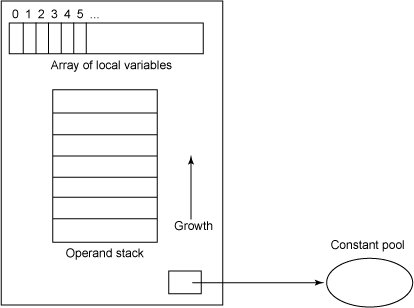
\includegraphics[width=240pt]{frame.jpg}}
\caption{Фрейм}\label{pic_Frame}
\end{figure}

Размер массива \textit{локальных переменных} определяется во время компиляции в зависимости от количества и размера локальных переменных и параметров метода. \textit{Стек операндов} --- LIFO-стек для записи и удаления значений в стеке; размер также определяется во время компиляции. Некоторые инструкции добавляют значения в стек, другие берут из стека операнды, изменяют их состояние и возвращают в стек. Стек операндов также используется для получения значений, возвращаемых методом. 

Каждый из потоков имеет свой \textit{регистр PC} (program counter). В любой точке каждый поток JVM выполняет код одного метода, называемого текущим методом этого потока. Если этот метод не нативный (native), то регистр PC содержит адрес JVM-инструкции, выполняющейся в данный момент. Если метод нативный, то значение регистра PC не определено. Размер регистра достаточно большой, чтобы содержать значение \texttt{returnAdress} или машинный указатель (native pointer) на специфической платформе.

В JVM есть \textit{куча}, которая разделена между всеми потоками. Куча --- это область данных времени выполнения (runtime data area), в которой расположены объекты классов и массивы. Куча создается при запуске виртуальной машины. Сборщик мусора занимается выделением памяти под объекты, удалением объектов и освобождением памяти.

Локальные переменные могут иметь типы \texttt{boolean}, \texttt{byte}, \texttt{char}, \texttt{short}, \texttt{int}, \texttt{float}, \texttt{reference} или \texttt{returnAdress}. Пара переменных может содержать значение типа \texttt{long} или \texttt{double}.

%Адреса локальных переменных индексированы. Индексация начинается с нуля. Целое число может быть индексом локальной переменной тогда и только тогда, когда оно не меньше нуля и меньше длины массива локальных переменных.

%Каждый фрейм содержит \textit{стек операндов}. Максимальная глубина стека определяется во время компиляции и добавляется вместе с кодом метода, ассоциированного с фреймом. Как только создается фрейм, его стек операндов пуст. JVM предоставляет инструкциям загружать константы и переменные из локальных переменных и полей на стек операндов. Другие инструкции берут операнды со стека, совершают инструкции над ними и кладут результат обратно на стек. Стек используется также для подготовки передачи параметров в методы и получения результатов. 

\subsection{Инструкции JVM}
Инструкции JVM состоят из однобайтового кода инструкции, за которым следуют ноль или более операндов в качестве аргументов. Некоторые данные, используемые в инструкции, передаются неявно через стек операндов. Перед инструкцией может стоять метка, на её можно ссылаться в переходах. Некоторые инструкции не имеют операндов и состоят только из кода инструкции. Многие инструкции имеют префиксы из одной буквы, соответствующие типам их операндов ({\it i} для операнда типа \texttt{int}, {\it l} для \texttt{long}, {\it s} для \texttt{short}, {\it b} для \texttt{byte}, {\it c} для \texttt{char}, {\it f} для \texttt{float}, {\it d} для \texttt{double}, и {\it a} для ссылки). Например, инструкция \texttt{iload} загружает содержимое локальной переменной, которая должна быть типа \texttt{int}, на стек операндов. В JVM не поддерживаются типы \texttt{boolean}, \texttt{byte}, \texttt{char} и \texttt{short}, вместо них используется тип \texttt{int}. 

%Например, инструкция \texttt{iadd} складывает два целых. Для этого ей необходимо, чтобы целые были в двух словах на вершине стека, помещенные туда предыдущими инструкциями. Оба целых извлекаются из стека, складываются, и их сумма помещается обратно в стек операндов. Промежуточные значения хранятся в стеке операндов, что обеспечивает поддержку вложенных вычислений.

Далее будут использоваться следующие обозначения. Знак ``\texttt{<n>}'' \space означает некоторое натуральное число. ``\texttt{x}'' \space в начале инструкции --- буква соответствующая типу (\textit{l, d, f, i} или \textit{a}). ``\texttt{<x>}''~--- число соответствующего типа. ``m1'' соответствует ``$-1$''.

\subsubsection*{Инструкции load и store}
Инструкции \texttt{load} и \texttt{store} перемещают значения между локальными переменными и стеком операндов фрейма. Среди них есть инструкции загрузки локальных переменных на стек операндов (\texttt{xload, xload\_<n>}), инструкции загрузки значений со стек операндов в локальные переменные (\texttt{xstore, xstore\_<n>}) и инструкции загрузки констант на стек операндов (\texttt{bipush, sipush, ldc, ldc\_w, ldc2\_w, aconst\_null, xconst\_m1, xconst\_<x>}). 

\subsubsection*{Арифметические операции}
Арифметические операции вычисляют значение по нескольким аргументам и кладут результат на стек операндов. Аргументов обычно два, и они заданы неявно через стек операндов. Арифметические операции делятся на два главных типа: оперирующие с целыми числами и оперирующие с числами с плавающей точкой. Любая из них реализована для конкретных численных типов JVM. Есть различия в поведении целочисленных и операций с числами с плавающей точкой при переполнении и делении на ноль. 

Существуют следующие арифметические операции: сложение (\texttt{xadd}), вычитание (\texttt{xsub}), умножение (\texttt{xmul}), деление (\texttt{xdiv}), взятие остатка (\texttt{xrem}), отрицание (\texttt{xneg}), двоичный сдвиг (\texttt{xshl, xshr, xushr}), поразрядное ИЛИ (\texttt{xor}), поразрядное И (\texttt{xand}), поразрядное исключительное ИЛИ (\texttt{xxor}), инкремент локальной переменной (\texttt{iinc}), сравнение (\texttt{xcmpg, xcmpl, lcmp}).

\subsubsection*{Инструкции приведения типов}
Для приведения типов в JVM есть следующие инструкции: \texttt{i2l}, \texttt{i2f}, \texttt{i2d}, \texttt{l2f}, \texttt{l2d}, and \texttt{f2d}. Левая буква означает тип, который приводят, правая --- тип к которому приводят. ``2'' означает ``to''. Например,  инструкция \texttt{i2d} приводит значение типа \texttt{int} в \texttt{double}.
  
\subsubsection*{Инструкции по управлению стеком операндов}
Набор инструкций для прямого управления стеком операндов:
\begin{itemize}
\item снятие верхнего значения со стека: \texttt{pop, pop2};
\item дублирование одного или двух значений на вершине стека: \texttt{dup, dup2, dup\_x1, dup2\_x1, dup\_x2, dup2\_x2};
\item обмен местами двух значений на вершине стека: \texttt{swap}.
\end {itemize}

\subsubsection*{Инструкции переходов}
%Инструкции потока управления условно или безусловно заставляют JVM продолжать выполнение с инструкции отличной от следующей инструкции потока управления. Вот они:
Среди инструкций переходов бывают:
\begin{itemize}
\item Условные переходы
\begin{itemize}
\item по сравнению с нулем: \texttt{ifeq, ifne, iflt, ifle, ifgt, ifge};
\item по сравнению с null: \texttt{ifnull, ifnonnull};
\item по сравнению двух операндов: \texttt{if\_icmpeq,if\_icmpne, if\_icmplt, if\_icmple, if\_icmpgt if\_icmpge, if\_acmpeq, if\_acmpne}.
\end{itemize}
\item Сложные условные переходы: \texttt{tableswitch, lookupswitch}.
\item Безусловные переходы: \texttt{goto, goto\_w, jsr, jsr\_w, ret}.
\end{itemize}
Переходы происходят по меткам, находящимися перед началом JVM-инструкции.

\subsubsection*{Вызов метода и инструкция return}
Существуют пять инструкций вызова метода: \texttt{invokevirtual, invokeinterface, invokespecial, invokestatic, invokedynamic}.

Инструкция возврата управления может быть без типа (\texttt{return}) или с типом (\texttt{xreturn})
%Инструкции return в методе, отличные от типа return: \texttt{ireturn}(используется для возврата значений типа \texttt{boolean, byte, char, short,} или \texttt{int}), \texttt{lreturn, freturn, dreturn,} и \texttt{areturn.}
\subsubsection*{Инструкции с полями}
Существуют две инструкции взятия значения из поля и две инструкции сохраняющие в поле: \texttt{getfield, getstatic, setfield, setstatic}.
\newpage
\subsection{Пример кода на JVM}
Для примера возьмем простую программу на Java и скомпилированный код на JVM.
\iffalse
\lstset{ %
language=java,                 % выбор языка для подсветки (здесь это С)
basicstyle=\small\sffamily, % размер и начертание шрифта для подсветки кода
numbers=left,               % где поставить нумерацию строк (слева\справа)
numberstyle=\tiny,           % размер шрифта для номеров строк
stepnumber=1,                   % размер шага между двумя номерами строк
numbersep=5pt,                % как далеко отстоят номера строк от подсвечиваемого кода
backgroundcolor=\color{white}, % цвет фона подсветки - используем \usepackage{color}
showspaces=false,            % показывать или нет пробелы специальными отступами
showstringspaces=false,      % показывать или нет пробелы в строках
showtabs=false,             % показывать или нет табуляцию в строках
frame=single,              % рисовать рамку вокруг кода
tabsize=2,                 % размер табуляции по умолчанию равен 2 пробелам
captionpos=t,              % позиция заголовка вверху [t] или внизу [b] 
breaklines=true,           % автоматически переносить строки (да\нет)
breakatwhitespace=false, % переносить строки только если есть пробел
escapeinside={\%*}{*)}   % если нужно добавить комментарии в коде
}
\fi

%\begin{figure} [h]
%\caption{Простой Java-класс}
\begin{lstlisting}[label=Java-example,caption=Простой Java-класс, frame = single, language = Java]
public class Example {
    private int f = 1; 

    public int foo(int p1, int p2) {
        return p1 + p2 - f;
    }

    public static void main() {
        Example ex = new Example();
        int p1 = 1, p2 = 2;
        int a = 3, c = 4;
        if (a < c)  ex.foo(p1, p2);
    }

    public int getF() {
        return f;
    }
}
\end{lstlisting}
%\end{figure}

Следующий код на JVM мы получим из скомпилированного класса Example.class с помощью дизассемблера javap. Так выглядит код, который необходимо декомпилировать (см. листинг \ref{JVM-example}).

%\begin{figure}
%\caption{Представление класса в JVM}
\newpage
\begin{lstlisting}[label=JVM-example,caption=Представление класса в JVM, frame = single, language = Java]
public class Example {
  public Example();
       0: aload_0
       1: invokespecial #1                  // Method java/lang/Object."<init>":()V
       4: aload_0
       5: iconst_1
       6: putfield      #2                  // Field f:I
       9: return

  public int foo(int, int);
       0: iload_1
       1: iload_2
       2: iadd
       3: aload_0
       4: getfield      #2                  // Field f:I
       7: isub
       8: ireturn

  public static void main();
       0: new           #3                  // class Example
       3: dup
       4: invokespecial #4                  // Method "<init>":()V
       7: astore_0
       8: iconst_1
       9: istore_1
      10: iconst_2
      11: istore_2
      12: iconst_3
      13: istore_3
      14: iconst_4
      15: istore        4
      17: iload_3
      18: iload         4
      20: if_icmpge     30
      23: aload_0
      24: iload_1
      25: iload_2
      26: invokevirtual #5                  // Method foo:(II)I
      29: pop
      30: return

  public int getF();
       0: aload_0
       1: getfield      #2                  // Field f:I
       4: ireturn
}
\end{lstlisting}
%\end{figure}


\pagebreak
\section{Использованные технологии}
В данном разделе описаны два использованных в работе инструмента.
%Работать напрямую с \texttt{class} файлами трудно, поскольку они в двоичном коде. Для удобной работы с ними используются хорошие инструменты.

\subsection{Библиотека ASM}
ASM\footnote{Официальная страница библиотеки ASM, \url{http://asm.ow2.org/}} \cite{asm_guide} --- многофункциональная библиотека для чтения и модификации JVM-классов. Для этого ASM предоставляет инструменты для чтения, записи и изменения байтовых массивов, которыми представлены классы, используя более высокоуровневые понятия: числовые константы, строки, идентификаторы, типы, классы, используемые в Java и т.д. 

Библиотека предоставляет два API для создания и изменения скомпилированных классов: API, дающее представление классов, основанное на событиях, и API, основанное на объектах. В нашей работе мы используем первый.

Модель, основанная на событиях, представлена последовательностью событий, каждое из которых представляет  элемент класса. Например, название класса, поле, описание метода, инструкция и т.д. Этот API определяет множество событий и порядок, в котором они должны произойти, и предоставляет парсер класса, создающий одно событие на каждый разобранный элемент.

%В начале идет построение дерева метаданных при помощи библиотеки ASM. Узлы дерева --- классы, поля и методы. Для их представления созданы классы, которые определяют особенности их описания и модификаторы доступа в соответствии с спецификацией виртуальной машины Java.

%Генерация кода осуществляется рекурсивным обходом в глубину дерева промежуточного представления. Мы это можем делать, поскольку иерархия дерева соответствует вложенности описания сущностей в исходном коде. Действительно, верно, что код из каждого объекта должен начать генерироваться раньше, чем из всех содержащихся в нем, а закончить после окончания генерации из них.

\subsection{Jasmin}
Jasmin\footnote{Официальная страница Jasmin - ассемблера для JVM,
\url{http://jasmin.sourceforge.net/}} --- ассемблер для JVM. На вход ему подаются описания классов, написанные в синтаксисе JVM. Он транслирует их в бинарные файлы, подходящие для исполнения на JVM. 

Jasmin может быть использован для создания \texttt{class}-файлов, которые нельзя было бы создать, скомпилировав Java-класс.

\pagebreak
\section{Декомпиляция выражений}
Целью курсовой работы является реализация декомпилятора выражений байт-кода JVM. Для этого сначала нужно понять, каким условиям должен удовлетворять код и, как частный случай, выражения на JVM. На код JVM накладываются синтаксические ограничения и ограничения верификации, т.е. проверки корректности класс-файла JVM. Будем рассматривать только такие выражения, которые удовлетворяют этим требованиям.

\subsection{Верификация}
Поскольку байт-код может быть создан не только компилятором javac, порождающий корректный байт-код, но и   другими средствами (библиотеки (ASM, BCEL\footnote{Официальная страница BCEL. Инструмент для работы с байт-кодом, \url{http://commons.apache.org/proper/commons-bcel/}}, SERP\footnote{Официальная страница SERP. Инструмент для работы с байт-кодом, \url{http://serp.sourceforge.net/}} для создания классов из байт-кода, компиляторы других фирм, Java-ассемблеры), необходима проверка корректности или верификация. JVM проводит проверку байт-кода при загрузке в несколько этапов. 

На первом проходе происходит загрузка (loading). Здесь проверяется формат класс-файла (magic number, длина).

На втором проходе происходит связывание (linking). На этом проходе проверяется соблюдение правил использования модификатора final, наличие суперкласса (кроме java.lang.Object), формат пул констант и ссылки внутри него.

Третий проход представляет, собственно, верификацию на этапе связывания. Проверяется формат команд байт-кода, аргументы и индексы, аргументы при вызове метода, входы в обработчики исключений (только через исключение) и семантика команд. В проверку семантики команд входит соответствие типов во время присваивания значений полям класса, доступ к локальным переменным в методе и размер стека операндов метода, типы значений в нем. То же проверяется для локальных переменных.

Четвертый (и последний) проход является виртуальным, проходит на этапе выполнения инструкции. В нем проверяется, что тип переменной или сигнатура вызываемого метода совпадают с теми, которые записаны в вызывающем методе компилятором, и флаги доступа вызываемого методу разрешают доступ из вызывающего метода. То же происходит для переменных. На этом проходе также проверяется, что вызываемый методы или переменная, к которой производится доступ, действительно существует в соответствующем классе.

При декомпиляции выражений важно следующее. При разветвлении в коде в конце каждой ветви на стеке должен остаться одинаковый по типу и количеству набор значений. После любого прохода разветвления на стеке остается определенный набор значений. Эти значения могут быть использованы, например, как аргументы метода.

%Это необходимо для того, чтобы после слияния разветвления (при любом его проходе) был также одинаковый по типу и количеству значений набор, т.е однозначно определенный. 


%При декомпиляции выражений важно, что в случае разветвления в коде на стек должно быть положено(или снято) в каждой ветви одинаковое количество значений, причем одинаковых типов соответственно. Таким образом, чтобы после слияния разветвления на стеке должен быть одинаковый по размеру и типам набор значений, т.е однозначно определенный. Эти значения могут быть, например, использованы как аргументы метода.

\subsection{Виды выражений}
Выражение в байт-коде JVM может быть написано без использования переходов или с ними. В последнем случае в разных ветвях выполнения программы могут быть положены на стек JVM несколько значений, а обработка, т. е. снятие их со стека и выполнение некоторой инструкции, может быть выполнена уже после завершения разветвления кода. Поэтому в выражение может входить часть графа потока управления.

\subsection{Выражения, содержащие переходы}
В случае выражений с переходами необходимо анализировать часть графа потока управления. Есть несколько естественных условий и определенных требований, которые накладываются на код, соответствующий выражению. Граф должен быть ориентированным, без циклов, иметь одну начальную вершину и одну конечную. Каждый узел --- участок линейного кода. Ребро --- переход из одной линейной части в другую. Из каждого узла выходит не более двух ребер. Действительно, два ребра будет при условном переходе и одно ребро при безусловном (goto). Главное условие --- на параллельных участках стек обрабатывается одинаковым образом. В конечной вершине величина стека может быть любой отличной от нуля (иначе это уже не выражение).

\subsubsection*{Пример выражения с переходами}
Ниже приведен пример корректного кода на JVM, который нельзя получить, скомпилировав Java-класс. Для удобства представления на рис. \ref{graph} изображен граф потока управления, соответствующий выражению. На нем показаны и пронумерованы участки линейного кода. Всего в графе девять вершин. Видно, что в коде четыре условных перехода (1, 2, 3, 5) и четыре безусловных перехода (4, 6, 7, 8). 

До вершины 1, на стек кладется объект класса graph (\texttt{28: aload\_0}). Потом перед каждым условным оператором кладутся на стек значение типа int для осуществления инструкции сравнения аргумента с нулем. В участках кода, соответствующих вершинам 4, 5 и 6, на стек кладутся два значения типа \texttt{int}. В участке 9 вызывается метод \texttt{foo} при трёх значениях на стеке: первое из них --- объект класса graph, от которого вызывается метод, остальные два значения типа \texttt{int}. После вызова метода на стеке остается одно значение.

\begin{lstlisting}[label=graph-example,caption = Пример кода выражения в JVM с переходами, frame = single, language = JAVA]
       8: new           graph                  
      11: dup
      12: invokespecial graph.<init>()V                 
      15: astore_0
      16: iconst_1
      17: istore_1
      18: iconst_2
      19: istore_2
      20: iconst_3
      21: istore_3
      28: aload_0  
      29: iload         2  ; vertex 1
      32: ifgt          58 
      33: iload_2          ; vertex 2
      35: ifle          65 
      36: iload_2          ; vertex 4     
      38: iload_3
      40: goto          80 
      58: iload_3          ; vertex 3
      60: ifge          82 
      65: iload_1          ; vertex 5
      66: iload_2
      67: iload_3
      70: ifle          90     
      80: goto          100 ; vertex 7
      82: iload_1           ; vertex 6
      84: iload_3
      85: goto          90
      90: goto          100 ; vertex 8
      100: invokevirtual graph.foo(II)I ;vertex 9
\end{lstlisting}

\begin{figure} [h]
\center{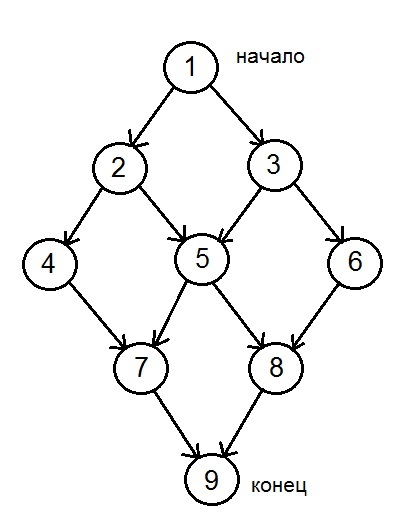
\includegraphics[width=130pt]{graph.jpg}}
\caption{Граф потока упраления, соответствующий выражению}\label{graph}
\end{figure}

Этот код действительно нельзя получить из Java, поскольку при вызове метода параметры загружаются на стек прямо перед вызовом метода. А в данном примере это происходит гораздо раньше. Мы могли бы получить эквивалентный код в Java только вызвав три раза метод \texttt{foo} при разных параметрах в разных ветках условных переходов. 

Такой вид выражений требуют глубокого анализа кода. Перед декомпиляцией его необходимо трансформировать в эквивалентный код на JVM, подходящий для промежуточного представления. Декомпиляция такого вида выражений пока не реализована. 

\subsection{Выражения, не содержащие переходы}
Будет рассмотрен разбор участка кода без переходов, который оставляет на стеке после себя одно значение, при нулевом начальном состоянии стека. 

\subsubsection*{Пример выражения без переходов}
Код JVM, соответствующий выражению, не содержащий переходов, можно получить из высокоуровневых языков. Например, скомпилировав Java-класс. Ниже в листинге \ref{java-example} приведен пример кода на Java соответствующий выражению. Его байт-код (приведен в листинге \ref{jvm-example}) декомпилируется созданным декомпилятором. 

\begin{lstlisting}[label=java-example,caption = Пример кода выражения в Java без переходов, frame = single, language = JAVA]
	int c = 1; 
 	int d = 3; 
	Example ex=new Example();
 	double b = ((c + d) * 3 - ex.foo(c,d)) / 10 + c*d; 
\end{lstlisting}

\begin{lstlisting}[label=jvm-example,caption = Пример кода выражения в JVM без переходов, frame = single, language = JAVA]
       0: iconst_1
       1: istore_0
       2: iconst_3
       3: istore_1
       4: new           #3                  // class Example
       7: dup
       8: invokespecial #4                  // Method "<init>":()V
      11: astore_2
      12: iload_0
      13: iload_1
      14: iadd
      15: iconst_3
      16: imul
      17: aload_2
      18: iload_0
      19: iload_1
      20: invokevirtual #5                  // Method foo:(II)I
      23: isub
      24: bipush        10
      26: idiv
      27: iload_0
      28: iload_1
      29: imul
      30: iadd
      31: i2d
      32: dstore_3
      33: return
\end{lstlisting}

Получается следующий код (выбранный целевой язык --- Java) при декомпиляции (листинг \ref{decompiled-example}). Этот код совпадает с исходным, что и требуется при построении декомпилятора.

\begin{lstlisting}[label=decompiled-example,caption = Пример кода выражения в JVM без переходов, frame = single, language = JAVA]
	int c = 1; 
	int d = 3; 
	Example ex = new Example();
	double b = ((c + d) * 3 - ex.foo(c,d)) / 10 + c * d; 
\end{lstlisting} 

\subsubsection*{Реализация}
В программе декомпилятора используется событийная модель анализа кода из библиотеки ASM. Эта модель создает событие и передает управление в метод, управляющий таким событием, когда при обходе байт-кода встречается определенная языковая конструкция. В этой модели есть \texttt{MethodVisitor}, анализирующий методы, и \texttt{ClassVisitor}, анализирующий классы. Для декомпиляции выражений используется функциональность \texttt{MethodVisitor}:
\begin{itemize}
\item \texttt{visitInsn} для обработки инструкций без операндов (их большинство);
\item \texttt{visitIntInsn} для обработки инструкций с одним операндом;
\item \texttt{visitVarInsn} для инструкций с локальными переменными;
\item \texttt{visitMethodInsn} для вызовов методов;
\item \texttt{visitJumpInsn} для обработки инструкций переходов.
\end{itemize}

Для представления выражения создан абстрактный класс \texttt{Expression}, от которого унаследованы разные классы видов выражений: бинарные, унарные, константы, вызовы функций, инструкция \texttt{new}. В бинарных и унарных выражениях есть, соответственно, левое и правое подвыражение или одно подвыражение. Они и составляют структуру JVM-дерева.

Для создания JVM-дерева используется стек выражений, получаемый из стека операндов. Каждое значение на стеке операндов --- это значение некоторого выражения. Когда встречается инструкция с двумя аргументами, значениями на стеке операндов, тогда снимается два верхних выражения со стека выражений и кладется на стек новое выражение, соответствующее данной инструкции и имеющее в качестве подвыражений предыдущие два. Если встретилась загрузка константы или переменной, то на стек кладется выражение, соответствующие константе или переменной. 

При вызове метода со стека снимаются столько значений, сколько аргументов у метода. Далее в зависимости от вида вызова метода на стек кладется либо выражение вызова обычного метода (при этом сначала еще со стека снимается объект, от которого вызывается метод), статического, конструктора или метода суперкласса. Внутри выражений для методов хранятся их аргументы в виде подвыражений.

Из-за того что на стеке операндов в конце рассматриваемого участка кода лежит одно значение, то и на стеке выражений будет храниться одно выражение, соответствующее этому значению.

\pagebreak
\section*{Заключение}
\addcontentsline{toc}{section}{Заключение}

В рамках курсовой работы разработан декомпилятор выражений по байт-коду JVM. При этом декомпилируемый код должен обладать следующими свойствами:
\begin{itemize}
\item Код проходит верификацию.
\item Часть кода, соответствующая выражению, является линейной без использования условных и безусловных переходов.
\item Выражение начинается с пустого стека.
\item Выражение заканчивается при глубине стека, равного 1. Это значение и является значением выражения.
\item Могут быть использованы арифметические инструкции, загрузка, выгрузка, снятие значения на стеке, вызов метода, инструкции с полями класса. 
\end{itemize}
Для представления выражений создается абстрактное дерево в терминах JVM. В узлах хранятся сущности, соответствующие инструкциям, потомки узлов --- подвыражения, соответствующие операндам инструкции.

\pagebreak
\bibliographystyle{ugost2008ls}
%\bibliography{expression}

\begin{thebibliography}{}
\bibitem{jvms}
Tim Lindholm, Frank Yellin, Gilad Bracha, Alex Buckley.
The Java Virtual Machine Specification.
Java SE 7 Edition, 2013. \\
\url{docs.oracle.com/javase/specs/jvms/se7/jvms7.pdf}

\bibitem{asm_guide}
Eric Bruneton.
ASM 4.0 A Java Bytecode Engineering Library. \\
\url{http://download.forge.objectweb.org/asm/asm4-guide.pdf}

\bibitem{book:suif}
Robert Wilson, Robert French, Christopher Wilson, Saman Amarasinghe, Jennifer Anderson. The SUIF Compiler System: a Parallelizing and Optimizing Research Compiler. 1994. Computer Systems Laboratory, Stanford University. \\ \url {http://dl.acm.org/citation.cfm?coll=GUIDE&dl=GUIDE&id=891422/}
\end{thebibliography}
\end{document}
